\beginsong{Was geh'n euch meine Lumpen an}[wuw={Barthel Schiers, Bruno Traven}, pfiii={69}, bo={360} index={Was geh'n euch meine Lumpen an}]

\markboth{\songtitle}{\songtitle}

\beginverse
\endverse

\centering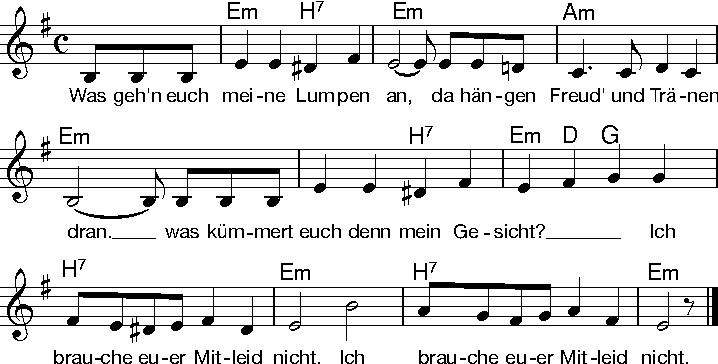
\includegraphics[width=1\textwidth]{Noten/Lied091.pdf}

\beginverse
Was kümmert \[Em]euch, was \[H7]mir ge\[Em]fällt, ich liebe \[Am]mich, nicht euch in dieser \[Em]Welt.
In euren Himmel \[H7]will ich \[Em]gar\[D]nicht \[G]rein, 
\lrep viel \[H7]lieber in der Hölle \[Em]sein. \rrep
\endverse


\beginverse
Ich brauch' ge^wiss nicht ^eure ^Gnaden, und selbst wenn ^Tote ich ge^laden,
wenn Schimpf und Schande ^wären ^an ^mir ^dran, 
\lrep das ^geht euch einen Scheißdreck ^an. \rrep
\endverse
\beginverse
Ich pfeife ^auf das ^Weltge^richt, an Aufer^stehung glaub ich ^nicht,
ob's Götter gibt, das ^weiß ich ^^^nicht, 
\lrep und ^Höllenstrafen fürcht' ich ^nicht. \rrep
\endverse

\endsong

\beginscripture{}

\endscripture

\begin{intersong}

\end{intersong}